\section{Solution}
In this section we describe the key ideas behind our design, and the decisions we made during the design process.
\subsection{Sequential Implementation}
To implement a sequential filter we had to solve a number of problems. In between each data input, we have to do 32 multiply accumulate operations. Therefore we have to buffer the latest 32 input values in an array \texttt{data}, in which the 0th index contains $x(i)$ and the last value is $x(i -31)$. This can be seen at the top of figure ~\ref{fig:architecture}. So in each step, the new data value is supplied to \texttt{data}[0], and for all $1 \leq i \leq 31$ the value of \texttt{data}[$i$-1] is copied to \texttt{data}[$i$]. An alternative solution would be to create a ring buffer, in which we supply the input value to the $(n\bmod 32)$-th slot of \texttt{data}. We decided not to use this approach, because it would require an extra register to point to the latest variable, and an extra multiplexer to index the input wires of the array.\\
After the $n^{th}$ input is supplied we need to calculate $y(n)=\Sigma_{0\leq i \leq 31}(h(i)\cdot x(n-i))$. In our design this corresponds to $\Sigma_{0 \leq i \leq 31}(data[i] * h\_in[i])$.  

\begin{figure}
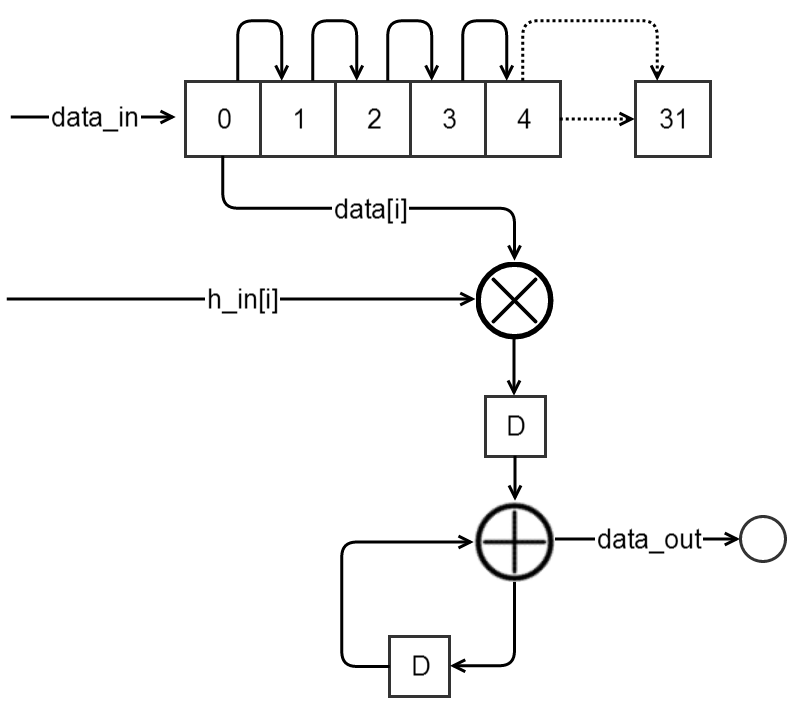
\includegraphics[width=0.9\textwidth]{images/architecture.png}
\caption{Architecture diagram of the sequential FIR filter.}
\label{fig:architecture}
\end{figure}
